
\documentclass[
12pt,
a4paper,
pdftex,
czech,
titlepage
]{report}
\usepackage{hyperref}
\usepackage[czech]{babel}
\usepackage[table]{xcolor}
\usepackage{array}
\usepackage[utf8]{inputenc}
\usepackage{lmodern}
\usepackage{textcomp}
\usepackage[T1]{fontenc}
\usepackage{amsfonts}
\usepackage{titlesec}
\usepackage{graphicx}
\usepackage{enumitem}
\usepackage{changepage}
\usepackage{csquotes}


\titleformat{\chapter}
  {\normalfont\LARGE\bfseries}{\thechapter}{1em}{}
\titlespacing*{\chapter}{0pt}{0ex plus 1ex minus .2ex}{2.0ex plus .2ex}

\begin{document}

\begin{titlepage}
	\vspace*{-2cm}
	{\centering
\includegraphics[scale=1.0]{logo.png}\par}
	\centering
	\vspace*{2cm}
	{\Large Semestrální práce z KIV/PC\par}
	\vspace{1.5cm}
	{\Huge\bfseries Algoritmus Minimax v deskové hře Othello\par}
	\vspace{2cm}

	{\Large Tomáš Vítek\par}
	{\Large A21B0316P\par}
	{\Large twitty@students.zcu.cz\par}

	\vfill

	{\Large 13.\,1.\,2024}
\end{titlepage}

\tableofcontents
\thispagestyle{empty}
\clearpage

\chapter{Zadání}
\setcounter{page}{1}
Naprogramujte v jazyce ANSI C přenositelnou1 \textbf{konzolovou aplikaci}, která umožní lidským
uživatelům či umělým inteligencím změřit si své síly v deskové hře \textbf{Othello}. Vámi implementovaná umělá inteligence bude pro zjištění optimálního
tahu využívat algoritmus \textbf{Minimax} rozšířený o tzv. \textbf{Alfa-beta prořezávání}. Jednotlivé hry bude
možné uložit a případně později načíst v definovaném formátu do textového souboru. Podoba
konzolového rozhraní je plně ve vaší kompetenci.

Program bude spouštěn příkazem othello.exe
s následujícím seznamem nepovinných argumentů
– výrazy v lomených závorkách (<>), resp. hranatých závorkách ([]) označují povinné, resp. nepovinné argumenty:

\begin{itemize}[label={}]
\item -pb <desc>
\hspace{1cm} \begin{minipage}[t]{0.7\textwidth} Popis hráče s černými kameny. Povinný argument <desc> popisující hráče
má strukturu "<human/minimax>[,name][,d]", kde human, resp. minimax
označuje lidského hráče, resp. umělou inteligenci (výchozí: human), name
představuje jméno hráče ve hře (výchozí: "Anna", případně "Karel"), nakonec výraz d určuje hloubku rozhodovacího stromu vytvářeného algoritmem
Minimax (výchozí: 3). Speciálně v případě hloubky stromu d = 0 algoritmus vždy vybere možný tah s postupně nejmenším číslem řádku a sloupce. V případě
lidského hráče bude hodnota d ignorována. Pokud je popis hráče zadán nesprávně, tj. jméno hráče není vyplněno nebo není unikátní, či hloubka
stromu není ostře větší než nula, program vypíše chybové hlášení ``Invalid player description!\textbackslash n'' a vrátí hodnotu 1.
\end{minipage}
\item -pw <desc>
\hspace{1cm} \begin{minipage}[t]{0.7\textwidth} Inicializace hráče s bílými kameny. Obdobně jako v případě přepínače -pb
\end{minipage}
\item -size <r> <c>
\hspace{0.6cm} \begin{minipage}[t]{0.7\textwidth} Argumenty r a c označují počet řádků a sloupců hracího pole. Hra na
obrázku 1 byla inicializována s hodnotami r = 8 a c = 7. Výchozí hodnoty
jsou r = 8 a c = 8. Pokud hodnoty argumentů r a c nejsou ostře větší než
1 (není kam umístit počáteční kameny), program vypíše chybové hlášení
``Invalid board size!\textbackslash n''
a vrátí hodnotu 2.
\end{minipage}
\item -init <ir> <ic>
\hspace{0.8cm} \begin{minipage}[t]{0.7\textwidth}  Na počátku hry jsou na hrací pole umístěny 4 kameny ve schématu ukázaném na obrázku 1. Argumenty ir a ic poté označují pozici prvního kamene. V případě hry na obrázku 1 byly hodnoty nastaveny ir = 5 a ic = 3.
Výchozí hodnoty jsou ir = 4 a ic = 4. Pokud není možné kameny na uvedenou pozici umístit, program vypíše chybovou hlášku ``Unable to place
initial stones!\textbackslash n'' a vrátí hodnotu 3.
\end{minipage}
\item -o <gamefile>
\hspace{1.05cm} \begin{minipage}[t]{0.7\textwidth} Do souboru gamefile bude v předepsaném formátu uložen aktuální stav
hry. Uložení bude provedeno automaticky na konci hry (když je znám vítěz hry) nebo v jejím průběhu zadáním příkazu "save". Do souboru budou
ukládány pouze akce hráčů, tj. speciální příkazy interpretu "save" a "quit"
budou ignorovány. Pokud umístění souboru gamefile není zapisovatelné,
program vypíše chybové hlášení ``Invalid output file destination!\textbackslash n''
a vrátí návratovou hodnotu 4. Výchozí hodnotou je prázdný řetězec.
\end{minipage}
\item -i <gamefile>
\hspace{1.1cm} \begin{minipage}[t]{0.7\textwidth}  Hra může být inicializována pomocí vstupního souboru gamefile, který
má totožnou strukturu jako v případě přepínače -o. Popis hry uvedený
v souboru gamefile může být přepsán argumenty -pb, -pw, -size nebo
-init. Pokud vstupní soubor gamefile nelze číst, program vypíše chybové
hlášení 
``Invalid input file!\textbackslash n'' a vrátí návratovou hodnotu 5. Výchozí
hodnotou je prázdný řetězec.
\end{minipage}
\end{itemize}

Vámi vyvinutý program tedy bude vykonávat následující činnosti:

\begin{enumerate}[label=\arabic*.]
\item Při spuštění bez přepínače -i <gamefile> bude hra inicializována argumenty -pb, -pw,
-size a -init a dále pokračovat v \textit{interaktivním režimu}, tj. postupně čekat na vstupy obou
hráčů. Zadané příkazy vyhodnotí a bude vyžadovat další, dokud nebude hra dokončena
nebo nebude uveden příkaz "quit". Při zadání chybného výrazu bude vypsána odpovídající
chybová hláška a hráč bude vyzván k opětovnému zadání vstupu.
\item Při spuštění s přepínačem -i <gamefile> bude hra načtena ze souboru <gamefile>. V souboru uvedené inicializační hodnoty je možné přepsat přepínači -pb, -pw, -size nebo -init.
Součástí vstupního souboru bude i seznam akcí obou hráčů a příkazů interpretu, které budou
dávkově zpracovány. Pokud během zpracování příkazů nedojde k chybě nebo k ukončení hry
(dokončením hry nebo uvedením příkazu "quit"), přejde aplikace do interaktivního režimu,
ve kterém budou hráči moci hru dokončit. Pokud během zpracování příkazů dojde k chybě,
program vypíše odpovídající chybovou hlášku a vrátí dedikovaný chybový kód.
\end{enumerate}

Hotovou práci odevzdejte v jediném archivu typu ZIP prostřednictvím automatického odevzdávacího a validačního systému. Postupujte podle instrukcí uvedených na webu předmětu. Archiv nechť
obsahuje všechny zdrojové soubory potřebné k přeložení programu, \textbf{Makefile} pro Windows i Linux
(pro překlad v Linuxu připravte soubor pojmenovaný Makefile a pro Windows Makefile.win)
a dokumentaci ve formátu PDF vytvořenou v typografickém systému \TeX (\LaTeX). Bude-li některá
z částí chybět, kontrolní skript Vaši práci odmítne.

\section*{Specifikace vyhodnocovaných výrazů
}
Výrazem může být pouze příkaz interpretu, nebo akce hráče. Interpret je \textbf{case-insesitive}, tj. nerozlišuje velká a malá písmena (zadané výrazy budou převedeny na malá písmena).
\newline\newline
Použití příkazů interpretu nebude zapsáno do výstupního souboru zadaného přepínačem -o. Příkazy ovšem budou vyhodnoceny, pokud se vyskytnou v souboru vstupním, který je dán přepínačem
-i. Interpret bude pracovat s následující minimální množinou podporovaných příkazů:
\begin{itemize}[label={}]
\item save
\hspace{0.5cm} \begin{minipage}[t]{0.8\textwidth}  Pokud je zadán výstupní soubor (přepínač -o), uloží do něj aktuální stav hry. V opačném případě neprovede žádnou akci. Pokud se uložení stavu hry do výstupního souboru
nepodaří, program vypíše chybové hlášení "Invalid output file destination!\textbackslash n"
a v případě režimu dávkového zpracování vrátí s návratovou hodnotou 4.
\end{minipage}

\item quit
\hspace{0.5cm} \begin{minipage}[t]{0.8\textwidth} Ukončí program s návratovou hodnotou EXIT\_SUCCESS.
\end{minipage}
\end{itemize}
Hráči se během hry střídají (začíná hráč s černými kameny) v zadání svých akcí, které postupně
mění stav hry. Akce hráčů budou nabývat následujících hodnot

\begin{itemize}[label={}]
\item <r>\_<c>
\hspace{0.5cm} \begin{minipage}[t]{0.7\textwidth}  Hráč umisťuje svůj kámen na pole v řádku r a sloupci c. V případě, že se jedná
o neplatný tah, program vypíše chybové hlášení 
``Invalid move!\textbackslash n''. Pokud k neplatnému tahu dojde navíc při načítání hry ze souboru, program skončí s návratovou
hodnotou 10.
\end{minipage}

\item pass
\hspace{0.8cm} \begin{minipage}[t]{0.8\textwidth} Ve hře může nastat situace, kdy hráči nezbývají žádné možné validní tahy. V takovém
případě zahraje tzv. pass. Pokud ale validní tah existuje, pak musí táhnout, i kdyby
to pro něj bylo nevýhodné. Na neplatném využití této akce reaguje program stejným
způsobem jako v případě <r>\_<c>.
\end{minipage}
\end{itemize}

\section*{Specifikace formátu vstupních a výstupních souborů}
Vstupní a výstupní soubory budou mít stejnou strukturu. V první části souboru budou v blocích
(hranatých závorkách) uvedeny hodnoty inicializačních argumentů \textbf{-pb, -pw, -size} nebo \textbf{
-init}.
Bezprostředně po bloku \textbf{"[game]"} bude následovat seznam hráči provedených akcí nebo příkazů
interpretu. Ukázku vstupního a výstupního souboru můžete vidět na konzolovém rozhraní 2.


\section*{Specifikace konzolového rozhraní}
Konzolové rozhraní aplikace je plně ve vaší kompetenci a nebude tedy validátorem kontrolováno.
Kvalita rozhraní bude zhodnocena 3 body. Například tedy při překreslování hracího pole po každém
tahu včetně výpisu aktuálního hráče apod. získáte 3 bodů. Oproti tomu minimální konzolové
rozhraní, tj. hra „naslepoÿ jenom s příkazovou řádkou bude nutně znamenat nulový bodový zisk.

\hfill {Vaší fantazii se v tomto případě meze nekladou!}

\section*{Algoritmus Minimax}
Vámi implementovaná umělá inteligence bude pro určení optimálního stavu využívat algoritmus
Minimax (společně s jeho vylepšením Alfa-beta prořezávání). V rámci detailní analýzy jistě zjistíte,
že algoritmus Minimax využívá k ohodnocení konkrétních stavů hry funkci, jejíž výpočet bude
v tomto případě
\[
    eval(s) = maxstones(s) - minstones(s),
\]
kde maxstones(s), resp. minstones(s) označuje počet kamenů maximalizujícího, resp. minimalizujícího hráče ve stavu s. V rámci analýzy problému navrhněte lepší hodnotící funkci, nežli je
navržená funkce eval(s).
Dbejte na to, aby akce (hrany stromu), které je možné v různých stavech hry provést, byly zleva
seřazeny postupně podle čísla řádku a sloupce taženého kamene. V případě, že algoritmus nalezne
více stavů maximalizujících hodnotu funkce eval, vaše implementace vždy vybere akci nejvíce
vlevo.

\chapter{Analýza úlohy}

\section{Zadání}
Zadání úlohy vyžaduje naprogramování konzolové přenositelné aplikace v jazyce \textbf{ANSI C}. Jejím obsahem bude implementace deskové hry \textbf{Othello} pro dva hráče, lidské či počítačově simulované skrze algoritmus \textbf{Minimax} rozšířený o \textbf{Alfa-beta prořezávání}.

\section{Othello}
Othello, taktéž znamé pod jménem Reversi, je desková hra pro dva hráče. Hráči používají černé a bílé kameny na své rozlišení. 

Cílem hry je získat na šachovnici více kamenů než má soupeř. Toho se docílí přeskakováním soupeřových kamenů ve všech 8 osměrech, tedy horizontálně, vertikálně i diagonálně. Každý tah musí být přeskočením některého ze soupeřových kamenů na prázdné políčko, pokud takový tah není k dispozici, hráč se svého tahu musí vzdát, pokud k dispozici je, hráč jej musí provést. Důležité je, že pokud lze na jedno políčko táhnout z více směrů, provedou se všechny tyto tahy současně.  

\section{Minimax}

Minimax je algoritmus, používaný pro hraní strategických her mezi dvěma a více hráči. Principem algoritmu je procházení stavového stromu hry a minimalizace maximálních možných ztrát. Algoritmus bývá základem většiny počítačových programů pro hraní her, jako jsou piškvorky, dáma, šachy nebo právě Othello.

Narozdíl od člověka nemůže algoritmus fungovat na základě metody "kouknu a vidím", ale je potřeba zkoumané prvky, tedy jednotlivé stavy hry, nějak kvantifikovat a ohodnotit. Volba způsobu ohodnocení je stěžějní pro získání nejlepších možných výsledků. Volba samozřejmě nikdy není jediná správná, v další podkapitole jich bude několik ukázáno. 

V momentě, kdy máme ohodnocené stavy hry, můžeme přistoupit k jejich prohledávání a porovnávní mezi sebou navzájem.

K tomu již lze použít algoritmus minimax, který funguje na principu prohledávání do hloubky. Vytváří strom všech možných tahů do určité hloubky a následně vybírá takový tah, který má nejlepší užitek pro hráče.

\begin{figure}[h]
  \centering
  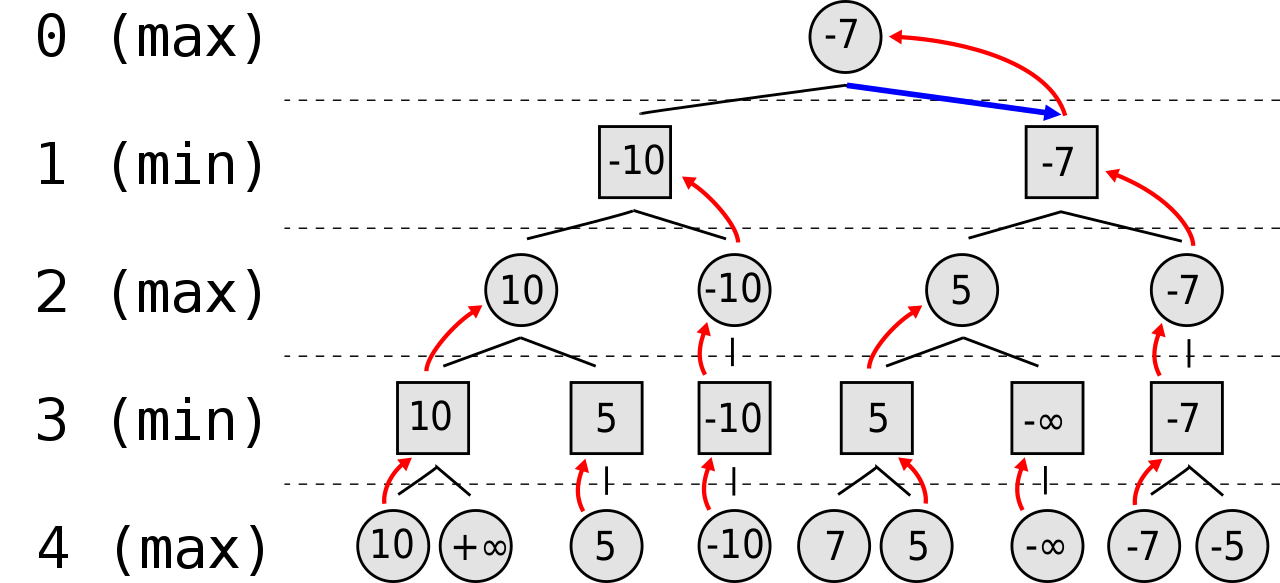
\includegraphics[scale=0.3]{min.png}
  \caption{Minimax}
\end{figure}

Takto by například vypadal stavový prostor agloritmu minimax do hloubky čtyři. Algorimtus začne provonávat hodnoty ze čtvrté úrovně z levé strany. Do třetí úrovně vybere hodnotu nejnižší ze čtvrté úrovně, do druhé úrovně hodnotu nejvyšší ze třetí úrovně, do první úrovně vybere hodnotu nejnižší ze druhé úrovně a konečně do nulté úrovně vybere hodnotu nejvyšší z první úrovně.

Je tomu tak proto, že sudé úrovně, tedy ta úplně první a potom pokaždé ob úroveň, patří hráči, jehož nejlepší tah hledáme. Ten se samozřejmě snaží získat co nejvyšší množství políček. Naproti tomu liché úrovně patří soupeři, ten by jistě také chtěl své políčka rozmnožit, proto vybíráme minimum, tedy naší největší ztrátu. Tak docílíme výběru nejlepšího možného tahu.

\subsection{Volba způsobu ohodnocení}

Způsoby ohodnocení možných tahů mohou být v každé úloze nejrůznější a ani pro jednu úlohu nemusí existovat jedno nejlepší řešení. Každá strategie může být jinak účinná na každého protivníka, uveďme si alespoň několik příkladů takových funkcí.

\subsubsection{Preference maximálního zisku polí}
Tato funkce ohodnotí daný tah dle změny v počtu políček obou hráčů. Tuto změnu lze snadno vyčíslit prostým sečtením políček hráče na tahu a soupeřových a poté porovávním s předcházejícím stavem. Tahy, které táhnoucímu hráči zvyšují a soupeři snižují počet políček, budou samozřejmě preferovány.

Toto lze vyjádřit následovně, \[
    eval(s) = maxstones(s) - minstones(s),
\]
kde maxstones(s), resp. minstones(s) označuje počet kamenů maximalizujícího, resp. minimalizujícího hráče ve stavu s.

Tento způsob ohodnocení vyžaduje zadání, proto bude využito v implementaci. 

\subsubsection{Preference ideálních polí}

Další možná strategie je ohodnotit jednotlivá políčka hrací desky čísly, dle jejich výhodnosti. Některá políčka jsou typicky mnohem výhodnější než jiná, třeba pro svoji lépe chráněnou polohu, anebo protože umožňují tahy do více stran než jiné.

\begin{table}[th]
    \centering
    \begin{tabular}{cccccccc}
        \cellcolor{red!100} 20 &
        \cellcolor{red!60} 18 & 
        \cellcolor{red!50} 16 &
        \cellcolor{red!40} 14 &
        \cellcolor{red!50} 16 &
        \cellcolor{red!60} 18 &
        \cellcolor{red!100} 20 \\
        \cellcolor{red!60} 18 &
        \cellcolor{red!50} 16 &
        \cellcolor{red!40} 14 &
        \cellcolor{red!30} 12 &
        \cellcolor{red!40} 14 &
        \cellcolor{red!50} 16 &
        \cellcolor{red!60} 18 \\
        \cellcolor{red!50} 16 &
        \cellcolor{red!40} 14 &
        \cellcolor{red!30} 12 &
        \cellcolor{red!20} 10 &
        \cellcolor{red!30} 12 &
        \cellcolor{red!40} 14 &
        \cellcolor{red!50} 16 \\
        \cellcolor{red!40} 14 &
        \cellcolor{red!30} 12 &
        \cellcolor{red!30} 12 &
        \cellcolor{red!10} 8 &
        \cellcolor{red!20} 10 &
        \cellcolor{red!30} 12 &
        \cellcolor{red!40} 14 \\
        \cellcolor{red!50} 16 &
        \cellcolor{red!40} 14 &
        \cellcolor{red!30} 12 &
        \cellcolor{red!20} 10 &
        \cellcolor{red!30} 12 &
        \cellcolor{red!40} 14 &
        \cellcolor{red!50} 16 \\
        \cellcolor{red!60} 18 &
        \cellcolor{red!50} 16 &
        \cellcolor{red!40} 14 &
        \cellcolor{red!30} 12 &
        \cellcolor{red!40} 14 &
        \cellcolor{red!50} 16 &
        \cellcolor{red!60} 18 \\
        \cellcolor{red!100} 20 &
        \cellcolor{red!60} 18 & 
        \cellcolor{red!50} 16 &
        \cellcolor{red!40} 14 &
        \cellcolor{red!50} 16 &
        \cellcolor{red!60} 18 &
        \cellcolor{red!100} 20 \\
    \end{tabular}
    \caption{Ohodnocení hracího pole 7x7}
    \label{tab:my_label}
\end{table}

Jedno z možných ohodnocení by mohlo být takovéto. Samotné rohy hrací desky jsou ohodnoceny nejvyšším číslem a políčka blížeji ke středu čím dál tím nižším číslem, ve středu hrací desky je ohodnocení zcela nejnižší.
Tato taktika je vhodná pro defenzivní hru.

\subsection{Alfa-Beta prořezávání}

Algoritmus minimax, jak již bylo uvedeno, je založen na grafovém algoritmu prohledávání do hloubky. Jelikož by ale stavový prostor například pro průměrnou šachovu partii obsahovala až $50^{100}$ možných stavů je v první řadě potřeba omezit tento strom co do hloubky.

I po tomto omezení však rozhodovací strom může být nadbytečně obsáhlý, proto je potřeba zredukovat nadbytečné stavy, k tomu se používá právě \textbf{Alfa-beta prořezávání}.

Jedná se o vylepšení algoritmu minimax, které v průměrném případě zrychluje jeho běh. Je založeno na pozorování, že pokud právě zpracovávaný tah už nemůže obstát v konkurenci s jiným, již nalezeným tahem, nemusíme dál prohledávat jeho důsledky. Tím se významně snižuje počet prohledávaných stavů.

Metoda byla pojmenována alfa-beta, protože v ní rozšiřujeme původní minimaxový algoritmus o dvě další hodnoty alfa a beta, které nám určují potřebné meze.
Alfa hodnota reprezentuje dolní mez ohodnocení tahu pro maximalizujícíhohráče. 
Beta hodnota představuje horní mez ohodnocení tahu pro minimalizujícho hráče. 

\begin{figure}[h]
  \centering
  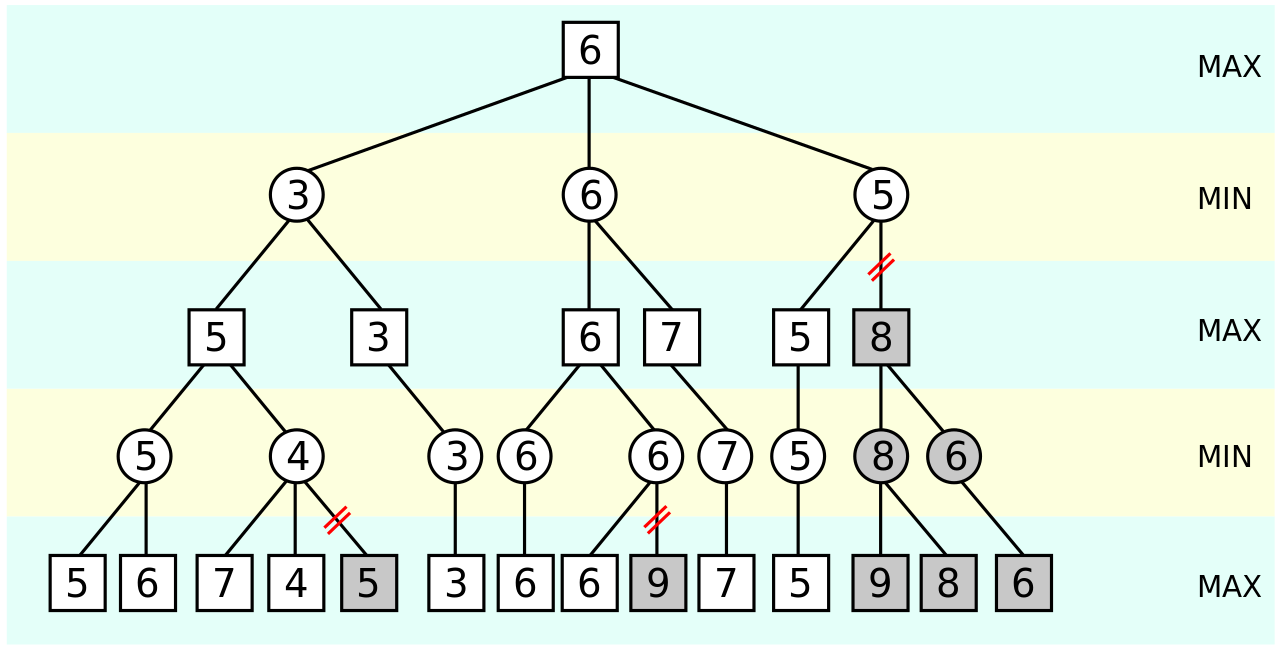
\includegraphics[scale=0.3]{AB.png}
  \caption{Alfa-beta prořezávání}
\end{figure}

Alfa-beta prořezávání by mohlo vypadat například takto. Šedou barvou je vyznačen stavový prostor, který již není potřebat prohledávat, protože již máme k dispozici lepší tah. 

Největší množství redukcí se typicky odehrává na pravé straně stavového prostoru, jelikož zde již máme dostupné informace, s kterými můžeme nově vzniklé porovnávat. 

\section{Hrací deska}
Podoba hrací desky není nijak přesně popsaná. Její velikost je dána skrz nepovinný parametr při spouštění:
\textit{-init <ir> <ic>}, kde první číslo udává počet řádků a druhé počet sloupců. Hrací deska je tedy nemá pevnou velikost a nemusí být nutně čtvercová.

Počet sloupců a řádků musí být vždy ostře větší než 1, horní mez bohužel není dána. Proto bude omezena velikostí datového typu \textit{int};
Konkrétní políčko na hrací desce může nést jen jednu hodnotu.

Hrací desku lze implemenovat jako 1D anebo 2D pole,které by bylo obecně lépe čitelné pro člověka, ale už složitěji implementovatelné. Tuto zkušenost jsem získal během programování šachů v předmětu KIV/UPG. Ve své implementaci zvolím cestu jednodimezionálního pole.

Za vhodné považuji vytvořit kolem hrací desky obal, který bude symbolizovat okraje desky. Zabrání se tak přetečení pole.

\section{Hráč}
Počet hráčů je pevně stanovený na dva. Hráčem může být buď člověk anebo počítač.

Hráče by bylo možné vytvořit jako dvě různé struktury, jedna pro minimax a druhá pro člověka. To by však mohlo zkompilokovat implementaci samotné hry. 

Jelikož se oba typy hráčů v mnohém neliší, budu je oba ukládat do stejné hráčské struktury, lidský hráč tedy přijme a uloží hloubku stromu, ale nebude jej nijak používat. 

\chapter{Popis implementace}

Projekt je implementován v jazyce \textit{ANSI C} za použití standartních knihoven \textit{<stdio.h>, <stdlib.h>, <ctype.h>} a \textit{<string.h>}.
Projekt je rozdělen do čtyř hlavičkových a sedmi .c souborů.

V souborech \textit{structure.h a structur.c} se nachází implementace všech potřebných struktur a funkcí k jejich alokaci, inicializaci, měnění obsahu jejich hodnot a další. 

Soubory \textit{reader.c, reader.h} obsahují implementaci načítání vstupních údajů od uživatele, ať už z příkazového řádku, tak ze souboru.
\textit{global.c} a \textit{global.h} slouží k deklaraci a inicializaci globálních proměnných dostupných kdekoliv v kódu. Jedná se především o instance obou hráčů, hracího pole a loggeru. Taktéž obsahují řadku preprocesových maker, pro přehlednost a snadnou změnu v kódu.

Implementace hry Othello je obsažena v souboru \textit{game.c}. 
Implementace algoritmu minimax je obsažena v souboru \textit{minimax.c}, svůj vlastní soubor má i logger v \textit{logger.c} a lidský hráč v \textit{human.c}. 

Hlavičkový soubor \textit{game.h} je společný pro soubory \textit{game.c, logger.c, minimax.c, human.c}

\section{Struktury}
Aplikace obsahuje tři struktury, \textit{hrací desku, hráče a logger}.
\subsection{Hrací deska}

Hrací deska je reprezentována struktoru board.
\begin{verbatim}
struct board {
    int rows;
    int cols;
    int size;
    int* values;
    int initX;
    int initY; 
    int K;
    int allDirections[8];
};
\end{verbatim}

Struktura uchovává informace o svojí velikosti, hodnot jednotlivých políček, počátečního rozložení políček, obsahuje i přepočet pro pohyb na desce a pole směrů, kterými se lze po hrací desce pohybovat.

Jelikož zde není žádný požadavek na konkrétní vizualizaci hrací desky ani rozložení kamenů, hrací deska bude vykreslena do konzole.  

Políčka na hrací desce jsou sice primárně určeny k tomu, aby byly nositely kamenů jednoho či druhého hráče, případně prázdné hodnoty. V mé implementaci jsem se rozhodl o využití i čtvrté hodnoty, která bude značit přesah za hrací pole, toto políčko bude zakázáno využít. Tím vznikne jakési obalení hrací desky hlídající validnost tahu a možné přetečení pole.

\subsection{Hráč}
Hráč, ať už lidský či počítačový, je posán struktoru player.

\begin{verbatim}
struct player {
    char *type; 
    char *name;
    int depth; 
    int symbol;
};
\end{verbatim}

Hráč má svoje jméno a rozlišení, jestli se jedná o lidského hráče, anebo algoritmus minimax. Taktéž si ukládá informace o hloubce stavového prostoru, kterou využívá jen počítačový hráč.
Na základě symbolu, lze rolišit černého a bílého hráče. Černý hráč má hodnotu symbolu vždy 1, bílý hráč je ohodnocen 2.

\subsection{Logger}

\begin{verbatim}
    struct logger {
    int capacity; 
    int upper_bar; 
    int bottom_bar; 
    char** move_char; 
    char* fileOutputName; 
};
\end{verbatim}

Logger spravuje záznamy o budoucích či minulých tazích. Jeho obsah je pak vypsán do výstupního souboru. 
Ukazatel \textit{upper\_bar} ukazuje na poslední tah, který byl právě odehrán. Ukazatel \textit{bottom\_bar} ukazuje na první tah, který dosud nebyl vypsán do výstupního soboru.

Kromě toho uchovává i informaci o názvu výstupního souboru.

\section{Důležité funkcionality}
Aplikace sestává z desítek různých funkcí, ty nejdůležitější vypadají takto.  
\subsection{Main funkce}
Vstupní bod aplikace, skládající se z načtení vstupních dat, jak z příkazové řádky tak ze vstupního souboru, spuštění hry a jejího ukončení včetně dealokace paměti.

\begin{verbatim}
    int main(int argv, char* argc[]){
    loadStartPoint(argv, argc);
    othello();
    ext(0);
    return 0;
}

\end{verbatim}

\subsection{Načítání vstupních dat}
Načítání vstupních dat ze souboru i z příkazové řádky obstarává stejná funkce \textit{load}. 

Z parametrů se prvně načítá vstupní soubor, pokud je připojen, poté velikost hrací desky a zbytek již v libovolém pořadí.
\begin{verbatim}
    void load(int argc, char *argv[], int fromFile) {
    int i;
    if(!argv || argc < 2){
        return;
    }
    prepareInputFile(argv, containsInputFile(argv,argc));
    containsSize(argc, (const char**) argv, fromFile);
    for (i = 1; i < argc; i++) {
        if (strcmp(argv[i], PB_TOKEN) == 0) {
            player1 = preparePlayer2(argv, i, BLACK);
        } else if (strcmp(argv[i], PW_TOKEN) == 0) {
            player2 = preparePlayer2(argv, i, WHITE);
        } else if (strcmp(argv[i], SIZE_TOKEN) == 0) {
            prepareSize(argv, i);
        } else if (strcmp(argv[i], INIT_TOKEN) == 0) {
            prepareInitBoard(argv, i);
        } else if (strcmp(argv[i], OUTPUT_TOKEN) == 0) {
            prepareOutputFile(argv, i);
        }
    }
}
\end{verbatim}

\subsection{Hra ze vstupu}
V situaci, kdy vstupní soubor obsahuje tahy hráčů, bude použita funkce \textit{inputplay()}. Jelikož jsou v loggeru tahy zapsány ve formátu X\_Y, je nutné si je prvně převést na číslo políčka, poté již jen zkoumáme, jestli je možné tah provést anebo jestli se jedná o jiný příkaz ze vstupního souboru. 

\begin{verbatim}
    int inputPlay(){
    int i,q, player; int* moves;
    if(logger == NULL || logger->capacity <= 0){
        return BLACK;
    }
    moves = malloc(sizeof (int* ) * logger->upper_bar);
    for(i = 0; i < logger->upper_bar; i++){
        moves[i] = transformInput(logger->move_char[i]);
    }
    i = 0; player = BLACK; q = logger->upper_bar;
    while(i < q){
        if(legalMove(moves[i], player, playboard->values)){ 
            makeMove(moves[i], player, playboard->values);
        } else if(moves[i] == -1 && !anyCorrectMove(player, playboard->values)) { 
            continue;
        }else if(moves[i] == -2){/
            printf("The game is over. Final result:\n");
            printboard();
            printToInputFile();
            ext(0);
        } else if(moves[i] == -3){ 
            printToInputFile();
            player = otherPlayer(player);
        } else {
                printf("Invalid move!\n");
                free(moves);
                ext(10);
            }
        printboard();
        i++;
        player = otherPlayer(player);
    }
    free(moves);
    return player;
}
\end{verbatim}
\subsection{Hraní hry}
Vstupním bodem do hry je funkce \textit{othello}, zde dochází především ke střídání hráčů a vypsání stavu hry uživateli, po provedení tahu.
\begin{verbatim}
    void othello () {
    int player;
    fillBoardByInnitValues(&playboard); /* Vložení inicializačních kamenů do hrací desky*/
    printboard();
    player = inputPlay();
    do {
        if (player == BLACK) {
            getmove(player1->type, BLACK, playboard->values);
        } else {
            getmove(player2->type, WHITE, playboard->values);
        }
        player = nextPlayer(playboard->values, player);
        printboard();
    }
    while (player != 0);
    printf("The game is over. Final result:\n");
    printboard();
    printToInputFile();
}
\end{verbatim}

\subsubsection{getMove}
Rozhodne, jestli je možné provést nějaký tah. Pokud ano, rozhodne zda hráč na tahu je minimax nebo člověk a vhodným způsobem se jej zeptá na tah.

\subsubsection{playMove}
Jako parametr získá chtěný tah, klasifikuje ho a rozhodne, jestli jej lze provést.

\subsection{makeMove}
Provede samotný tah. Z cílového políčka, označení hráče na tahu a stavu hrací desky provede všechny možné tahy.

\subsection{Minimax}
Funkcionalita algoritmu minimax je umístěna ve stejnojmeném .c souboru. 
\begin{verbatim}
int minimaxAB (int player, int * board, int depth, int alpha, int beta, char* type) {
    int i, max, nextPlay, newscore, bestmove, * arrayMoves, * newboard, size;
    if(!player || !board || depth < 0){
        return 0;
    }
    arrayMoves = validMoves(player, board); /* vytvoří všech pole validních tahů*/
    bestmove = -1;
    max = LOSS - 1;
    size = arrayMoves[0]; /* nultý index obsahuje počet tahů, zpravidla menší číslo než rozsah pole */;
    for (i = 1; i <= size; i++) {
        newboard = copyboard(board); /* vytvořá další pole, kde si vyzkoušíme daný scénář */
        makeMove(arrayMoves[i], player, newboard); /* Udělej můj tah */
        nextPlay = nextPlayer(newboard, player);
        if (nextPlay == 0) { /* Pokud již není validní tah */
            newscore = weightMove(player, newboard);
            if (newscore > 0) newscore = WIN;
            if (newscore < 0) newscore = LOSS;
        }
        newscore = minChoiceAB(player, newboard, depth - 1, alpha, beta, type); /*protivnikovy tahy*/
        if (newscore > max) { /*pokud mame lepsi tah nez je dosavad nejlepsi*/
            max = newscore;
            bestmove = arrayMoves[i]; /*ulozime si pozici nejlepsiho tahu*/
        }
        if (max >= beta) { /*pokud je nas nejlepsi tah lepsi nez WIN varianta*/
           free(newboard);
           break;
        }
       if (max > alpha) { /*hodnota nejlepsiho tahu je lepsi nez LOSS*/
            alpha = max;
        }
        free(newboard);
    }
    free(arrayMoves);
    return (bestmove);
}
\end{verbatim}

\subsection{minChoice}
Vrací minimální tah, simuluje tak rozhodnutí protihráče.
\subsection{maxChoice}
Vrací maximální tah, simuluje tak hráče na tahu.

\chapter{Uživatelská příručka}

\section{Struktura}
\section{Překlad}
Aplikace je pouze konzolová a je ji nutné nejprve přeložit, o což se stará soubor \textbf{Makefile}. Překlad se spouští příkazem \textit{make -f Makefile} na Linuxu, poté již lze aplikaci spustit. Pro spuštění na Windows je potřeba použít příkaz \textit{make -f Makefile.win}

\section{Spuštění}
Aplikaci lze spusit příkazem  \textit{.\othello.exe} Aplikace může být spuštěna pomocí parametrů \textit{-pb <desc> -pw <desc> -size <r> <c> -init <ir> <ic> -o <gamefile> -i <gamefile>}, nebo pouze s některými, parametry můžou být uvedeny ve zcela libovolném pořadí. Aplikace může být spuštěna bez jakéhokoliv parametru. Vstupní a výstupní soubory však musí být v .txt formátu.

Pro windows je spuštění stejné jako pro linux.

\section{Výstup}
Výstupem programu je konzolové zobrazení hrací desky. Případně vypsání chybového hlášení do konzole.
\begin{figure}[ht]
    \centering
    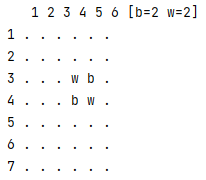
\includegraphics[width=0.4\linewidth]{othello.png}
    \caption{Grafický výstup programu}
    \label{fig:enter-label}
\end{figure}
\chapter{Závěr}
I přes všechny slepé cesty, a že jsem se po nich s nadšením vydal, se mi podařilo naprogramovat aplikaci, která splňuje požadavky zadání.

Projekt byl otestován, jak se zapnutým Alfa-beta přořezáváním (s A-B), tak bez něj (bez A-B), na prehisotrickým notebooku HP ProBook s 8GB RAM a 1.6 GHz. Počáteční pozice byla vždy ve středu hrací desky. Oba hráči byli řízeny algoritmem minimax se stejnou hloubkou stromu.
\begin{table}[ht]
    \centering
    \begin{tabular}{|c|c|c|c|}
        \hline
        Rozměr &  Hloubka & s A-B [s] & bez A-B [s]\\
        \hline
          4x4& 1& 0.001& 0.001\\
          4x4& 3& 0.001& 0.001\\
          4x4& 5& 0.001& 0.004\\
          4x4& 7&  0.003& 0.028\\
          \hline
          8x8 & 1 & 0.039 & 0.039\\
          8x8 & 3 & 0.090 & 0.258 \\
          8x8 & 5 & 0.317 & 4.463 \\
          8x8 & 7 & 6.794 & 916.364  \\
          \hline
          12x12 & 1 & 0.112& 0.112\\
          12x12 & 3 & 0.320 & 1.210 \\
          12X12 & 5 & 7.414 & 207.612 \\
          12x12 & 7 & 243.727 & +5h \\
        \hline
    \end{tabular}
    \caption{Délka běhu progamu}
\label{tab:my_label}
\end{table}
\newline  Z tabulky vyplývá, že alfa-beta prořezávání několikanásobně urychluje chod programu. 

Hra by mohla být vylepšena o grafické uživatelské rozhraní, které by ji učinilo atraktivnější pro uživatele. Po stránce funkcionality nevidím velký prostor pro zlepšení. Bylo by možné použít vhodnější ohodnocení hracího pole. Myslím, že je i dobře uzpůsobena pro změny v kódu.

\chapter{Zdroje}
\subsubsection{Literatura}
MASAŘÍK, V., ŠTĚPÁNKOVÁ, O., LAŽANSKÝ, J., Umělá inteligence (1), Academia, 1. vydání, 1993, ISBN-80-200-0496-3.
\subsubsection{Internetové zdroje}
\url{http://www.hrejsi.cz/othello/pravidla.htm}.

\chapter{Seznam vyobrazení}
\subsubsection{Tabulky}
 Tabulka 2.1: Ohodnocení hracího pole 7x7, vlastní vyobrazení,
\newline Tabulka 5.1: Délka běhu programu, vlasní vyobrazení.
\subsubsection{Obrázky}
Obrázek 2.1: Minimax, dostupné z: 
\url {https://en.wikipedia.org/wiki/Minimax},
\newline Obrázek 2.2: Alfa-beta prořezávání, dostupné z: \url{https://en.wikipedia.org/wiki/Alpha–beta_pruning},
\newline Obrázek 4.1: Grafický výstup programu, výstup z aplikace othello.exe.


\end{document}